\documentclass[a4paper,14pt]{extarticle}

% Путь до папки с общими шаблонами
\newcommand{\pathToCommonFolder}{/home/denilai/Documents/repos/latex/Common}
% Название работы в титуле
\newcommand{\workname}{Отчет по лабораторной работе №1}
% Название дисциплины в титуле
\newcommand{\discipline}{Проектирование и разработка систем на базе ПЛИС}
% Название кафедры в титуле
\newcommand{\kafedra}{Кафедра Вычислительной техники}
% Тема работы в титуле
\newcommand{\theme}{Проектирование синтезируемых моделей комбинационной
	логической схемы и их верификация средствами САПР Xilinx}
% Должность преподавателя в титуле
\newcommand{\rang}{ассистент}

% ФИО студента в титуле
\newcommand{\studentfio}{К.~Ю.~Денисов}
% ФИО преподавателя в титуле
\newcommand{\teacherfio}{А.~С.~Боронников}


\usepackage{tabularx}


\usepackage{booktabs}
\newcolumntype{b}{X}
\newcolumntype{s}{>{\hsize=.5\hsize}X}
\newcommand{\heading}[1]{\multicolumn{1}{c}{#1}}

% установка размера шрифта для всего документа
%\fontsize{20pt}{18pt}\selectfont
\usepackage{extsizes} % Возможность сделать 14-й шрифт

% Вставка заготовки преамбулы
% Этот шаблон документа разработан в 2014 году
% Данилом Фёдоровых (danil@fedorovykh.ru) 
% для использования в курсе 
% <<Документы и презентации в \LaTeX>>, записанном НИУ ВШЭ
% для Coursera.org: http://coursera.org/course/latex .
% Исходная версия шаблона --- 
% https://www.writelatex.com/coursera/latex/5.3

% В этом документе преамбула

% Для корректного использования русских символов в формулах
% пакеты hyperref и настройки, связанные с ним, стоит загуржать
% перед загрузкой пакета mathtext



% поддержка русских букв
% кодировка шрифта
%\usepackage[T2A]{fontenc} 
\usepackage{pscyr}

% использование ненумеровонного абзаца с добавлением его в содержаниеl

\newcommand{\anonsection}[1]{\section*{#1}\addcontentsline{toc}{section}{#1}}
\newcommand{\sectionunderl}[1]{\section*{\underline{#1}}}


% настройка окружения enumerate
\usepackage{enumitem}
\setlist{noitemsep}
\setlist[enumerate]{labelsep=*, leftmargin=1.5pc}

\usepackage{hyperref}

% сначала ставить \usepackage{extsizes} % Возможность сделать 14-й шрифт
% для корректной установки полей вставлять преамбулу следует в последнюю очередь (но перед дерективой замены \rmdefault)
\usepackage[top=20mm,bottom=25mm,left=35mm,right=20mm]{geometry} % Простой способ задавать поля

\hypersetup{				% Гиперссылки
	unicode=true,           % русские буквы в раздела PDF
	pdftitle={Заголовок},   % Заголовок
	pdfauthor={Автор},      % Автор
	pdfsubject={Тема},      % Тема
	pdfcreator={Создатель}, % Создатель
	pdfproducer={Производитель}, % Производитель
	pdfkeywords={keyword1} {key2} {key3}, % Ключевые слова
	colorlinks=true,       	% false: ссылки в рамках; true: цветные ссылки
	linkcolor=red,          % внутренние ссылки
	citecolor=black,        % на библиографию
	filecolor=magenta,      % на файлы
	urlcolor=blue           % на URL
}

%%% Работа с русским языком
\usepackage{cmap}					% поиск в PDF
\usepackage{mathtext} 				% русские буквы в формулах
\usepackage[T2A]{fontenc}			% кодировка
\usepackage[utf8]{inputenc}			% кодировка исходного текста
\usepackage[english,russian]{babel}	% локализация и переносы
\usepackage{indentfirst}
\frenchspacing

%для изменения названия списка иллюстраций
\usepackage{tocloft}


\renewcommand{\epsilon}{\ensuremath{\varepsilon}}
\renewcommand{\phi}{\ensuremath{\varphi}}
\renewcommand{\kappa}{\ensuremath{\varkappa}}
\renewcommand{\le}{\ensuremath{\leqslant}}
\renewcommand{\leq}{\ensuremath{\leqslant}}
\renewcommand{\ge}{\ensuremath{\geqslant}}
\renewcommand{\geq}{\ensuremath{\geqslant}}
\renewcommand{\emptyset}{\varnothing}

% Изменения параметров списка иллюстраций
\renewcommand{\cftfigfont}{Рисунок } % добавляем везде "Рисунок" перед номером
\addto\captionsrussian{\renewcommand\listfigurename{Список иллюстративного материала}}

\newcommand{\tm}{\texttrademark\ }
\newcommand{\reg}{\textregistered\ }


%%% Дополнительная работа с математикой
\usepackage{amsmath,amsfonts,amssymb,amsthm,mathtools} % AMS
\usepackage{icomma} % "Умная" запятая: $0,2$ --- число, $0, 2$ --- перечисление

%% Номера формул
%\mathtoolsset{showonlyrefs=true} % Показывать номера только у тех формул, на которые есть \eqref{} в тексте.
%\usepackage{leqno} % Нумереация формул слева

%% Свои команды
\DeclareMathOperator{\sgn}{\mathop{sgn}}

%% Перенос знаков в формулах (по Львовскому)
\newcommand*{\hm}[1]{#1\nobreak\discretionary{}
{\hbox{$\mathsurround=0pt #1$}}{}}


% отступ для первого абзаца главы или параграфа
%\usepackage{indentfirst}

%%% Работа с картинками
\usepackage{graphicx}  % Для вставки рисунков
\graphicspath{{images/}{screnshots/}}  % папки с картинками
\DeclareGraphicsExtensions{.pdf,.png,.jpg}
\setlength\fboxsep{3pt} % Отступ рамки \fbox{} от рисунка
\setlength\fboxrule{1pt} % Толщина линий рамки \fbox{}
\usepackage{wrapfig} % Обтекание рисунков текстом

%%% Работа с таблицами
\usepackage{array,tabularx,tabulary,booktabs} % Дополнительная работа с таблицами
\usepackage{longtable}  % Длинные таблицы
\usepackage{multirow} % Слияние строк в таблице

%%% Теоремы
\theoremstyle{plain} % Это стиль по умолчанию, его можно не переопределять.
\newtheorem{theorem}{Теорема}[section]
\newtheorem{proposition}[theorem]{Утверждение}

\theoremstyle{plain} % Это стиль по умолчанию, его можно не переопределять.
\newtheorem{work}{Практическая работа}[part]


 
 
\theoremstyle{definition} % "Определение"
\newtheorem{corollary}{Следствие}[theorem]
\newtheorem{problem}{Задача}[section]
 
\theoremstyle{remark} % "Примечание"
\newtheorem*{nonum}{Решение}



%%% Программирование
\usepackage{etoolbox} % логические операторы

%%% Страница

%	\usepackage{fancyhdr} % Колонтитулы
% 	\pagestyle{fancy}
%   \renewcommand{\headrulewidth}{0pt}  % Толщина линейки, отчеркивающей верхний колонтитул
% 	\lfoot{Нижний левый}
% 	\rfoot{Нижний правый}
% 	\rhead{Верхний правый}
% 	\chead{Верхний в центре}
% 	\lhead{Верхний левый}
%	\cfoot{Нижний в центре} % По умолчанию здесь номер страницы

\usepackage{setspace} % Интерлиньяж
\onehalfspacing % Интерлиньяж 1.5
%\doublespacing % Интерлиньяж 2
%\singlespacing % Интерлиньяж 1

\usepackage{lastpage} % Узнать, сколько всего страниц в документе.

\usepackage{soul} % Модификаторы начертания


\usepackage[usenames,dvipsnames,svgnames,table,rgb]{xcolor}


\usepackage{csquotes} % Еще инструменты для ссылок

%\usepackage[style=authoryear,maxcitenames=2,backend=biber,sorting=nty]{biblatex}

\usepackage{multicol} % Несколько колонок

\usepackage{tikz} % Работа с графикой
\usepackage{pgfplots}
\usepackage{pgfplotstable}

% модуль для вставки рыбы
\usepackage{blindtext}

\usepackage{listings}
\usepackage{color}


% для поворота отдельной страницы. Использовать окружение \landscape
\usepackage{pdflscape} 
\usepackage{rotating} 


\definecolor{mygreen}{rgb}{0,0.6,0}
\definecolor{mygray}{rgb}{0.5,0.5,0.5}
\definecolor{mymauve}{rgb}{0.58,0,0.82}


% пример импорта файла
%\lstinputlisting{/home/denilai/repomy/conf/distributions}

\lstset{
	language=Python,
	basicstyle=\footnotesize,        % the size of the fonts that are used for the code
	numbers=left,                    % where to put the line-numbers; possible values are (none, left, right)
	numbersep=5pt,                   % how far the line-numbers are from the code
	numberstyle=\tiny\color{mygray}, % the style that is used for the line-numbers
	stepnumber=2,                    % the step between two line-numbers. If it's 1, each line will be numbered
	% Tab - 2 пробела
	tabsize=2,    
	% Автоматический перенос строк
	breaklines=true,
	frame=single,
	breakatwhitespace=true,
	title=\lstname 
}



\author{Кирилл Денисов}
\title{Лабораторная работа №1}
\date{\today}

%если не нужна тема работы в отчете, то указать в скобках что-либо, иначе оаставить пустым
\renewcommand{\withouttheme}{fd}
%если нужна дата представления отчета, то указать в скобках что-либо
%\renewcommand{\withoutsubmissiondate}{1}

% установка полуторного интервала
% \usepackage{setspace}  
% \onehalfspacing

% использовать Times New Roman
\renewcommand{\rmdefault}{ftm}


\begin{document}
	\thispagestyle{empty}
	% Вставка первого титульного листа
	%\newcounter{withouttheme}

%\setcounter{withouttheme}{<n>} установить значение счетчика  withouttheme для определения, нужна ли тема
%    {0} - нужна
%    {1} - не нужна

%\setcounter{withoutsubmissiondate}{<n>} установить значение счетчика  withoutsubmissiondate для определения, нужна ли дата представления к защите
%     {0} - нужна
%     {1} - не нужена
\begin{center}
	\begin{figure}[h!]
		\begin{center}
		%\vspace{-10ex}
		
\includegraphics[width=0.17\linewidth]{\pathToCommonFolder/gerb}
		%\caption{}\label{pic:first}
		%	\vspace{5ex}
		\end{center}	
	\end{figure}
 	\small	МИНОБРНАУКИ РОССИИ \\
	Федеральное государственное бюджетное образовательное учреждение\\
						высшего образования\\
\normalsize					
\textbf{«МИРЭА – Российский технологический университет»\\
						РТУ МИРЭА}\\
						\noindent\rule{1\linewidth}{1pt}\\
       Институт информационных технологий\\ %\vspace{2ex}
					\kafedra\\
		\vspace{3ex}
			\large \textbf{\workname}  \\
		%\vspace{1ex}
						по дисциплине\\ «\discipline» \\
		\vspace{3ex}
		\ifnum \value{withouttheme}=0 {
			\textbf{Тема работы:}\\ <<\theme>>
		}
		\else {}
		\fi
\vspace{10ex}
\small
\begin{table}[h!]
\begin{tabular}{lp{0.6\linewidth}l}
	\textbf{Выполнил:} & студент группы ИВБО-02-19 & \\ 
	& & \studentfio \\%Д.~Н.~Федосеев\\%А.~М.~Сосунов\\%К.~Ю.~Денисов\\%И.~А.~Кремнев
	\textbf{Принял:} & \rang & \\
	& & \teacherfio \hfill\\
\end{tabular}
\end{table}
\end{center}
\ifnum \value{withoutsubmissiondate}=0 {
	\begin{flushleft}
		Работа представлена к защите <<\rule{3ex}{1pt}>>\rule{10ex}{1pt} 202\rule{1ex}{1pt} г.\hfill
	\end{flushleft}
\else {}
\fi

\normalsize
\begin{center}	
\vfill
Москва 2022
\end{center}

	\newpage
	\tableofcontents
	\newpage
	%\listoftables
\section{Ход работы}	
\subsection {Постановка задачи}
Спроектировать синтезируемые модели комбинационной схемы 4х4, описанной
таблицей истинности согласно варианту задания, тремя различными способами:
\begin{enumerate}
	\item На вентильном уровне, методом карт Карно в виде МДНФ, в схемотехническом
	редакторе Schematic editor САПР Xilinx ISE Design Suite.
	\item На вентильном уровне, методом карт Карно в виде МКНФ, на языке описания
	аппаратуры Verilog.
	\item На поведенческом уровне, на языке описания аппаратуры Verilog.
	Реализовать на языке Verilog тестовое окружение и провести верификацию
	спроектированных моделей при помощи симулятора iSim из состава
	САПР Xilinx ISE Design Suite.
\end{enumerate}

Провести апробацию моделей при помощи отладочной платы Digilent Nexys 4 на
ПЛИС Xilinx Artix 7 XC7A100T-1CSG324. Комбинации на входах комбинационных схем
должны задаваться при помощи движковых переключателей отладочной платы,
комбинации на выходах комбинационных схем должны отображаться светодиодами
отладочной платы.
\subsection {Индивидуальный вариант 149}
Спроектировать синтезируемые модели комбинационной схемы 4х4 согласно данной таблице истинности и вектор-функции (см. таблицу \ref{tab:func-vector}).

\begin{table}[htbp]
	\begin{center}
	\begin{tabular}{|c|c|c|c|c|c|c|c|c|c|c|c|c|c|c|c|}
		\hline
		F & E & D & C & B & A & 9 & 8 & 7 & 6 & 5 & 4 & 3 & 2 & 1 & 0 \\ \hline\hline
		0 & 4 & 4 & 8 & 3 & 0 & 7 & 2 & 2 & D & 7 & C & 5 & 2 & A & C \\ \hline
	\end{tabular}
	\caption{Вектор-функция}
	\label{tab:func-vector}
\end{center}
\end{table}
\subsection{Построение таблицы истинности}
Построим таблицу истинности по заданному вектору. Входы обозначим $X_3, X_2, X_1, X_0$, а выходы $Q_3$,  $Q_2$, $Q_1$,  $Q_0$ соответственно (см. таблицу \ref{tab:func-table}).

\newpage
\begin{table}[htbp]
	
\begin{center}
		\begin{tabular}{|c||c|c|c|c||c||c|c|c|c|}
		\hline
		№ & $X_3$ & $X_2$ & $X_1$ & $X_0$ & F & $Q_3$ & $Q_2$ & $Q_1$ & $Q_0$ \\ \hline \hline
		0 & 0 & 0 & 0 & 0 & c & 1 & 1 & 0 & 0 \\ \hline
		1 & 0 & 0 & 0 & 1 & a & 1 & 0 & 1 & 0 \\ \hline
		2 & 0 & 0 & 1 & 0 & 2 & 0 & 0 & 1 & 0 \\ \hline
		3 & 0 & 0 & 1 & 1 & 5 & 0 & 1 & 0 & 1 \\ \hline
		4 & 0 & 1 & 0 & 0 & c & 1 & 1 & 0 & 0 \\ \hline
		5 & 0 & 1 & 0 & 1 & 7 & 0 & 1 & 1 & 1 \\ \hline
		6 & 0 & 1 & 1 & 0 & 0 & 1 & 1 & 0 & 1 \\ \hline
		7 & 0 & 1 & 1 & 1 & 2 & 0 & 0 & 1 & 0 \\ \hline
		8 & 1 & 0 & 0 & 0 & 2 & 0 & 0 & 1 & 0 \\ \hline
		9 & 1 & 0 & 0 & 1 & 7 & 0 & 1 & 1 & 1 \\ \hline
		10 & 1 & 0 & 1 & 0 & 0 & 0 & 0 & 0 & 0 \\ \hline
		11 & 1 & 0 & 1 & 1 & 3 & 0 & 0 & 1 & 1 \\ \hline
		12 & 1 & 1 & 0 & 0 & 8 & 1 & 0 & 0 & 0 \\ \hline
		13 & 1 & 1 & 0 & 1 & 4 & 0 & 1 & 0 & 0 \\ \hline
		14 & 1 & 1 & 1 & 0 & 4 & 0 & 1 & 0 & 0 \\ \hline
		15 & 1 & 1 & 1 & 1 & 0 & 0 & 0 & 0 & 0 \\ \hline
	\end{tabular}
\end{center}
	\caption{Таблица истинности}
	\label{tab:func-table}
\end{table}

\subsection{Построение карт Карно}
Построим карты Карно для 4 переменных $X_3, X_2, X_1, X_0$ для каждой из бинарных функций $Q_3$,  $Q_2$, $Q_1$,  $Q_0$ (см. рис. \ref{ris:karno-maps}).

\begin{center}
	\begin{figure}
	\begin{minipage}[h]{0.47\linewidth}
		\center{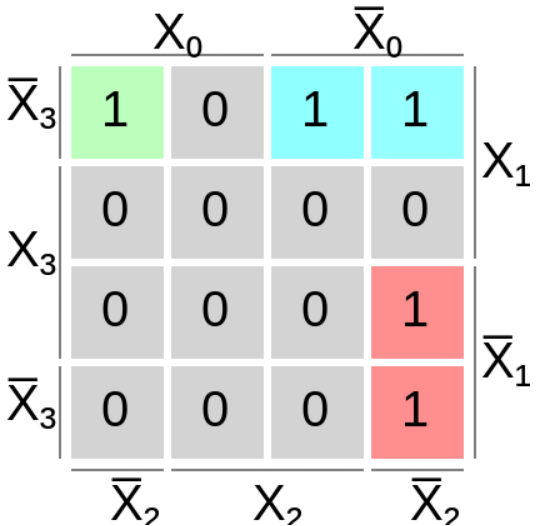
\includegraphics[width=1\linewidth]{images/y3}} а) \\
	\end{minipage}
	\hfill
	\begin{minipage}[h]{0.47\linewidth}
		\center{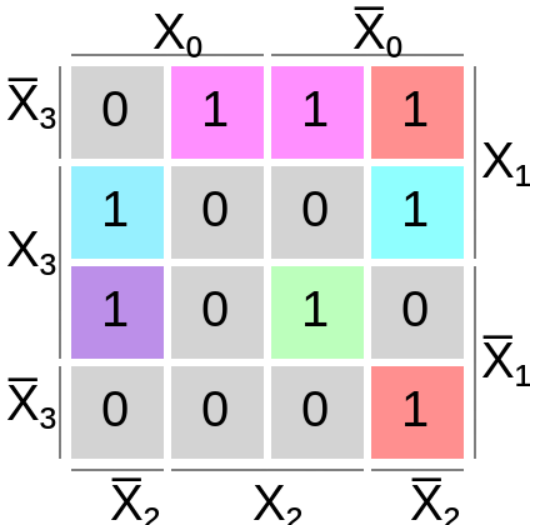
\includegraphics[width=1\linewidth]{images/y2}} \\б)
	\end{minipage}
	\vfill
	\begin{minipage}[h]{0.47\linewidth}
		\center{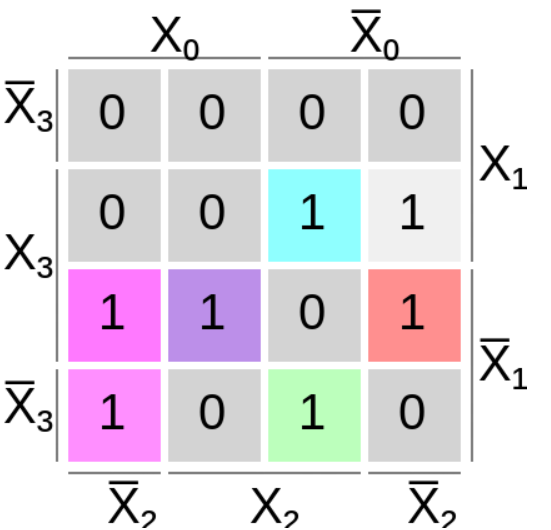
\includegraphics[width=1\linewidth]{images/y1}} в) \\
	\end{minipage}
	\hfill
	\begin{minipage}[h]{0.47\linewidth}
		\center{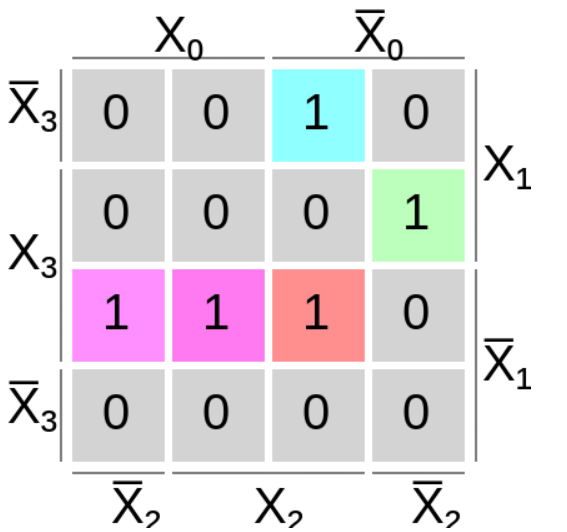
\includegraphics[width=1\linewidth]{images/y0}} г) \\
	\end{minipage}
	\caption{Карты Карно для 4-х переменных для функций а)$Q_3$, б)$Q_2$, в)$Q_2$, г)$Q_1$, д)$Q_0$}
	\label{ris:karno-maps}
\end{figure}
\end{center}

\subsection{Минимизация булевых функций}
По построенным картам Карно опишем \textbf{МДНФ} для реализации данных функций на вентильном уровне в редакторе Schematic editor САПР Xilinx ISE Design Suite.

\begin{align*}
	Q_3 &= \bar{X_3}\bar{X_2}\bar{X_1} \vee  X_2 \bar{X_1}\bar{X_0}  \vee \bar{X_3} X_2\bar{X_0} \\
	Q_2 &= \bar{X_3} \bar{X_1} \bar{X_0} \vee \bar{X_3} \bar{X_2} X_1 X_0 \vee X_2  \bar{X_1}  X_0 \vee X_2  X_1  \bar{X_0} \vee  X_3  \bar{X_1}  X_0 \\
	Q_1 &=  \bar{X_3}\bar{X_1}X_0    \vee  \bar{X_3} \bar{X_2} X_1 \bar{X_0} \vee     \bar{X_3} X_2  X_0  \vee  X_3 \bar{X_2} \bar{X_1}   \vee  X_3 \bar{X_2} X_0 \\
	Q_0 &= \bar{X_2} X_1 X_0 \vee \bar{X_3} X_2 \bar{X_1} X_0 \vee \bar{X_3} X_2 X_1 \bar{X_0} \vee X_3 \bar{X_2} X_0
 \end{align*}

Также опишем \textbf{МКНФ} для реализации булевых функций средствами VHDL в САПР Xilinx ISE Design Suite.
\begin{align*}
	Q_3 &=\left(
	\bar{X_3}\vee \bar{X_1}
	\right) 
	\cdot 
	\left(
	 X_2\vee \bar{X_1}
	 \right) 
	  \cdot  
	  \left(
	  \bar{X_2}\vee \bar{X_0}
	   \right) \\
	Q_2 &= \left(
	X_2 \vee X_2 \vee X_1 \vee \bar{X_0}
	\right) 
	\cdot 
	\left( 
	\bar{X_3} \vee X_2 \bar{X_1}
	 \right) 
	 \cdot 
	 \left(
	  X_2 \vee  \bar{X_1} \vee X_0
	   \right)
	    \cdot \\
	    & \left(
	    \bar{X_2}  \vee \bar{X_1} \vee \bar{X_0}
	    \right)
	     \cdot 
	      \left(\bar{X_3} \vee X_1 \vee X_0
	      \right)\\
	  Q_1 & = \left( X_3 \vee X_1 \vee X_0 \right) \cdot
	  \left( \bar{X_3} \vee \bar{X_1 X_0} \right) \cdot
	  \left( \bar{X_3} \vee \bar{X_2} \right) \cdot \\
	  & \left(X_3 \vee X_2 \vee \bar{X_1} \vee \bar{X_0}\right) \cdot
	  \left(\bar{X_2} \vee X_0\right)\\
	  Q_0 & = \left( X_3 \vee X_2 \vee X_1 \right) \cdot
	  \left(  X_2 \vee X_0 \right) \cdot
	  \left( X_1 \vee X_0  \right) \cdot
	  \left( \bar{X_3} \vee \bar{X_2} \right) \cdot
	  \left( \bar{X_2} \vee \bar{X_1} \vee \bar{X_0} \right)
\end{align*}
\subsection{Реализация функций в схемотехническом редакторе}
Опишем функции $Q_3$,  $Q_2$, $Q_1$,  $Q_0$ на вентильном уровне в схемотехническом редакторе Schematic editor САПР Xilinx ISE Design Suite (см. рис. \ref{fig:sheme1}, \ref{fig:sheme2}).

% TODO: \usepackage{graphicx} required
\begin{figure}[p]
	\centering
	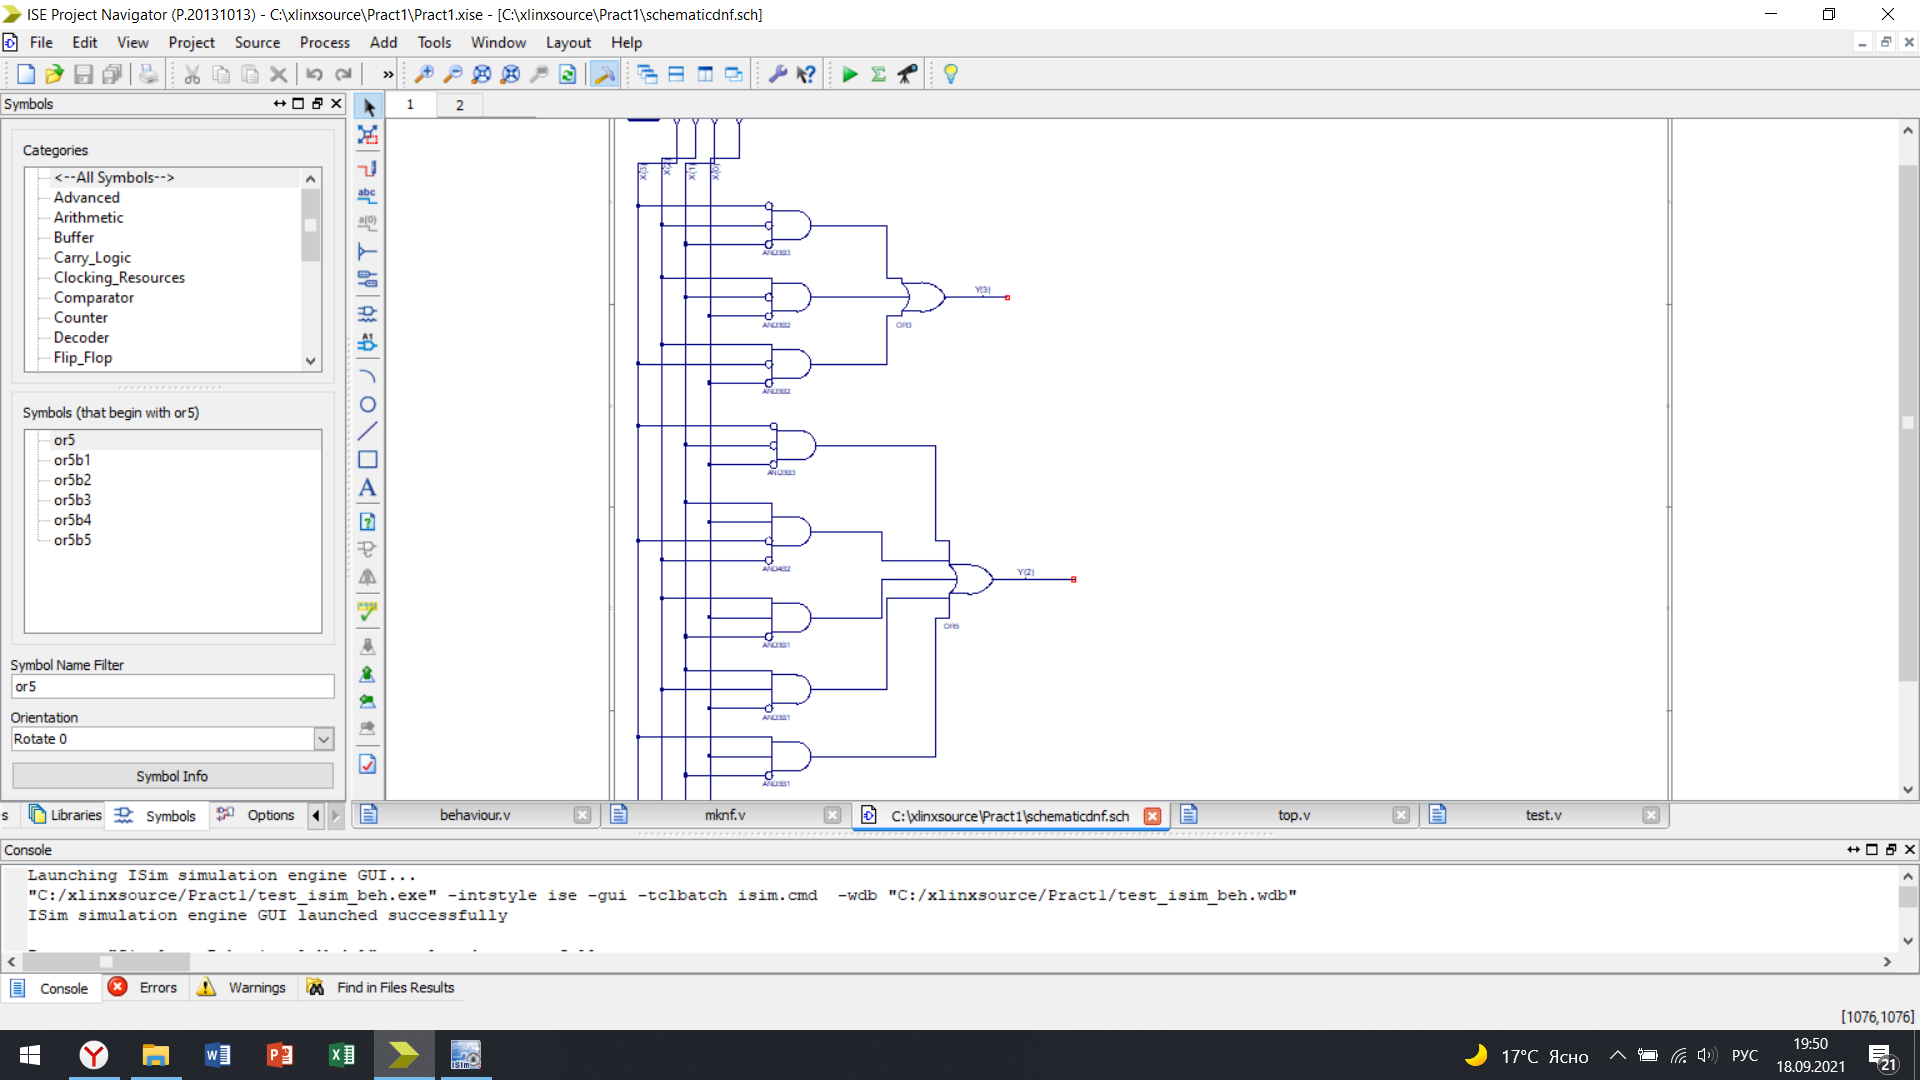
\includegraphics[width=\linewidth]{images/sheme1}
	\caption{Схемотехнический редактор. Лист 1}
	\label{fig:sheme1}
\end{figure}
%\newpage

% TODO: \usepackage{graphicx} required
\begin{figure}[p]
	\centering
	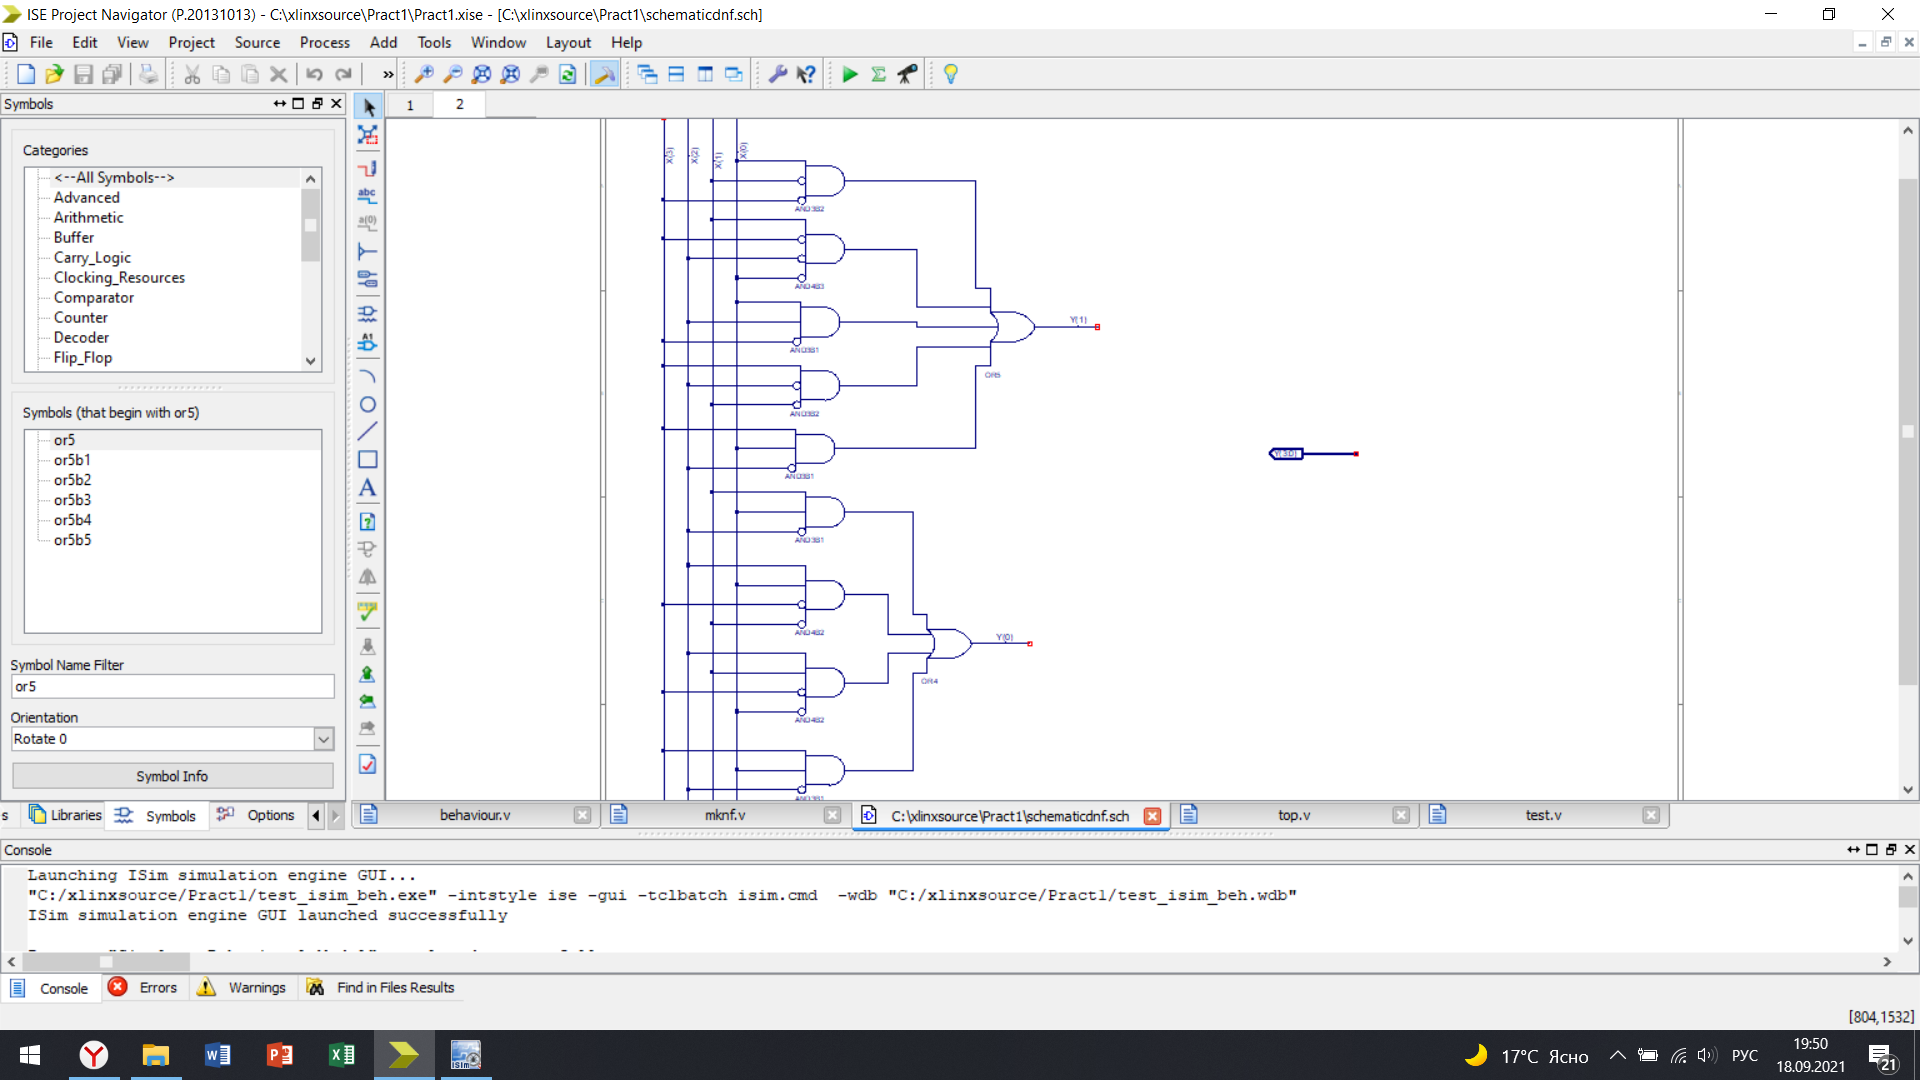
\includegraphics[width=\linewidth]{images/sheme2}
	\caption{Схемотехнический редактор. Лист 2}
	\label{fig:sheme2}
\end{figure}

\subsection{Реализация функций на вентильном уровне}
На основании МКНФ опишем функции $Q_3$,  $Q_2$, $Q_1$,  $Q_0$ на вентильном уровне c помощью языка Verilog.

\lstinputlisting{/home/denilai/Documents/repos/latex/scripts/mknf.v}

\newpage
\subsection{Реализация функций на поведенческом уровне}
На основании построенной ранее таблицы истинности (см. таблицу \ref{tab:func-table}) опишем функции $Q_3$,  $Q_2$, $Q_1$,  $Q_0$ на поведенческом уровне c помощью языка Verilog.
\lstinputlisting{/home/denilai/Documents/repos/latex/scripts/behaviour.v}

\newpage
\subsection{Создание проекта САПР Xilinx ISE}

Опишем файл верхнего уровня проекта САПР Xilinx ISE Design Suite, в котором подключим все остальные модули, укажем входные и выходные сигналы. 
\lstinputlisting{/home/denilai/Documents/repos/latex/scripts/top.v}


\subsection{Тестирование и отладка средствами симулятора iSim}
После компоновки проекта, подключения модуля верхнего уровня, проведем верификацию спроектированных моделей с помощью симулятора iSim из состава САПР Xilinx ISE Design Suite. Результаты тестирования можно видеть на рис. \ref{fig:test-result} и \ref{fig:isim}.

% TODO: \usepackage{graphicx} required
\begin{figure}[htpb]
	\centering
	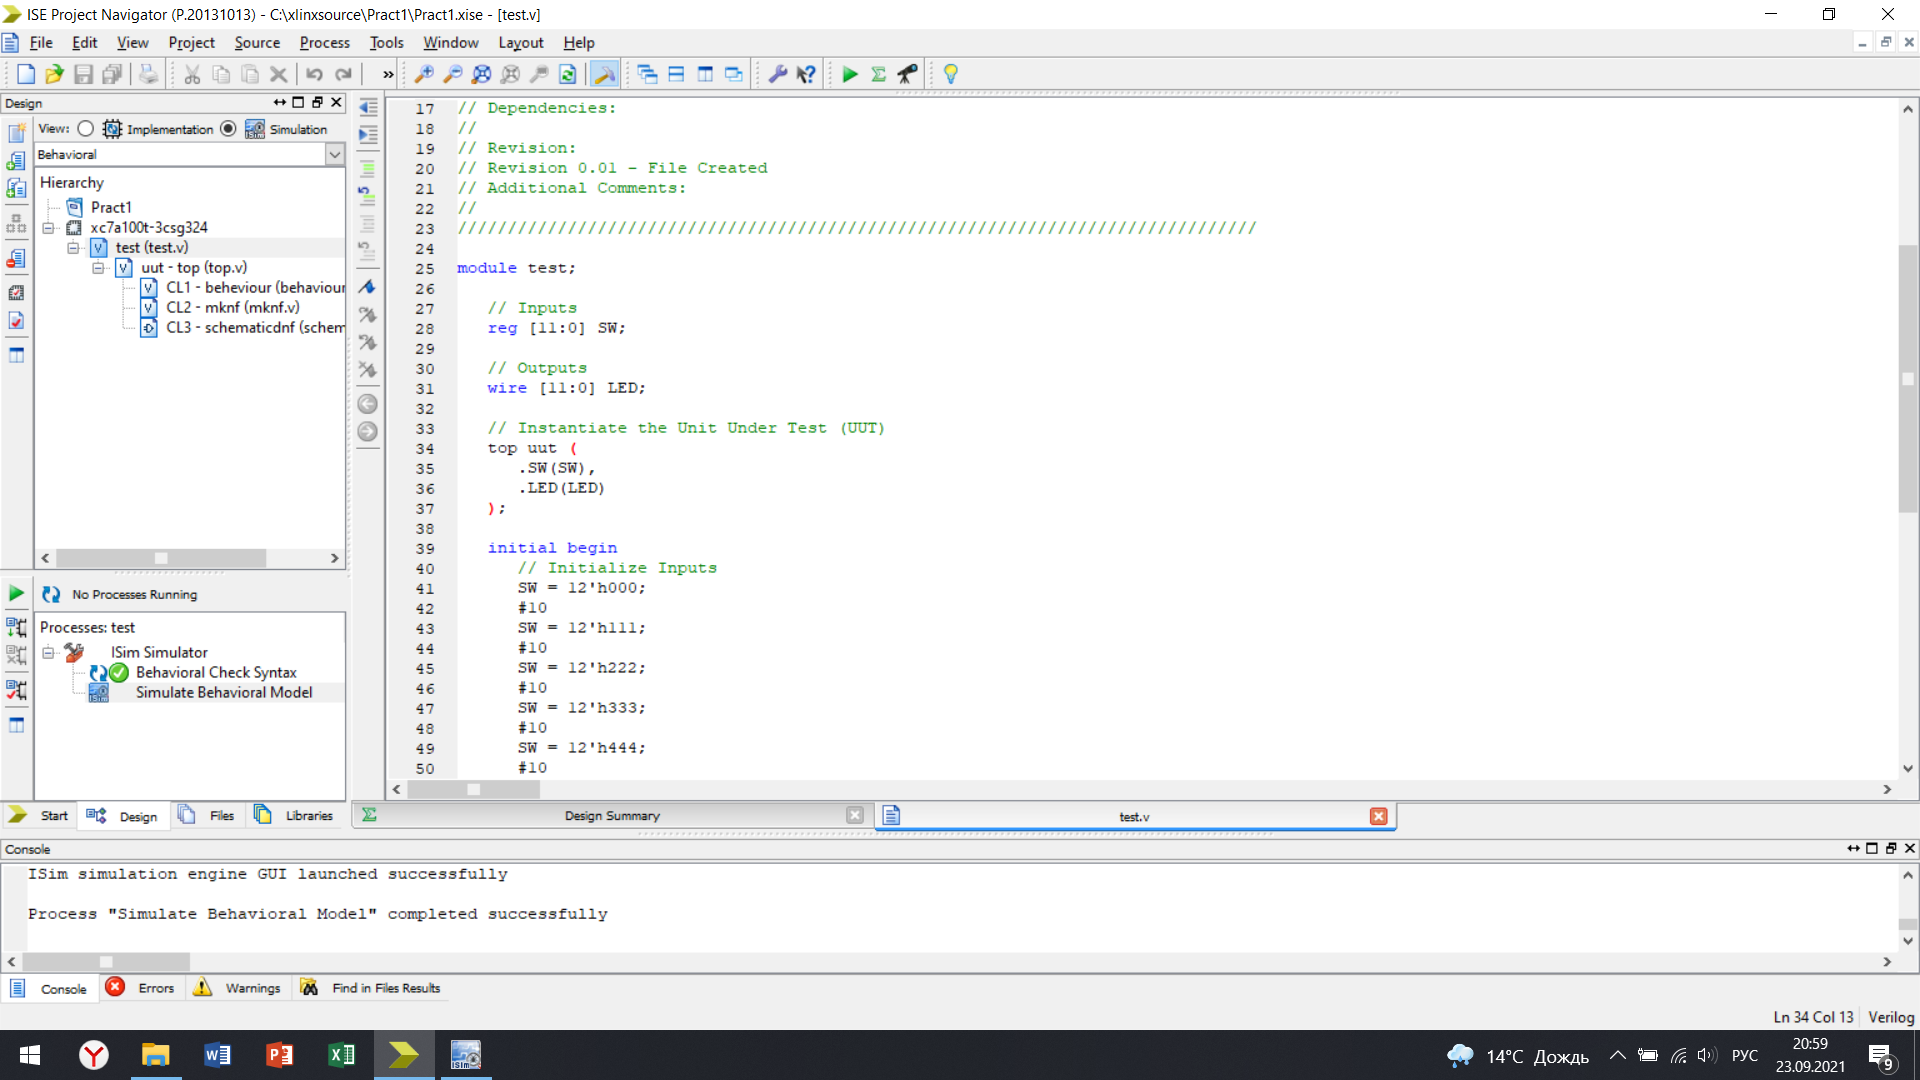
\includegraphics[width=\linewidth]{images/test-result}
	\caption{Проверка синтаксиса}
	\label{fig:test-result}
\end{figure}
% TODO: \usepackage{graphicx} required
\begin{figure}[htpb]
	\centering
	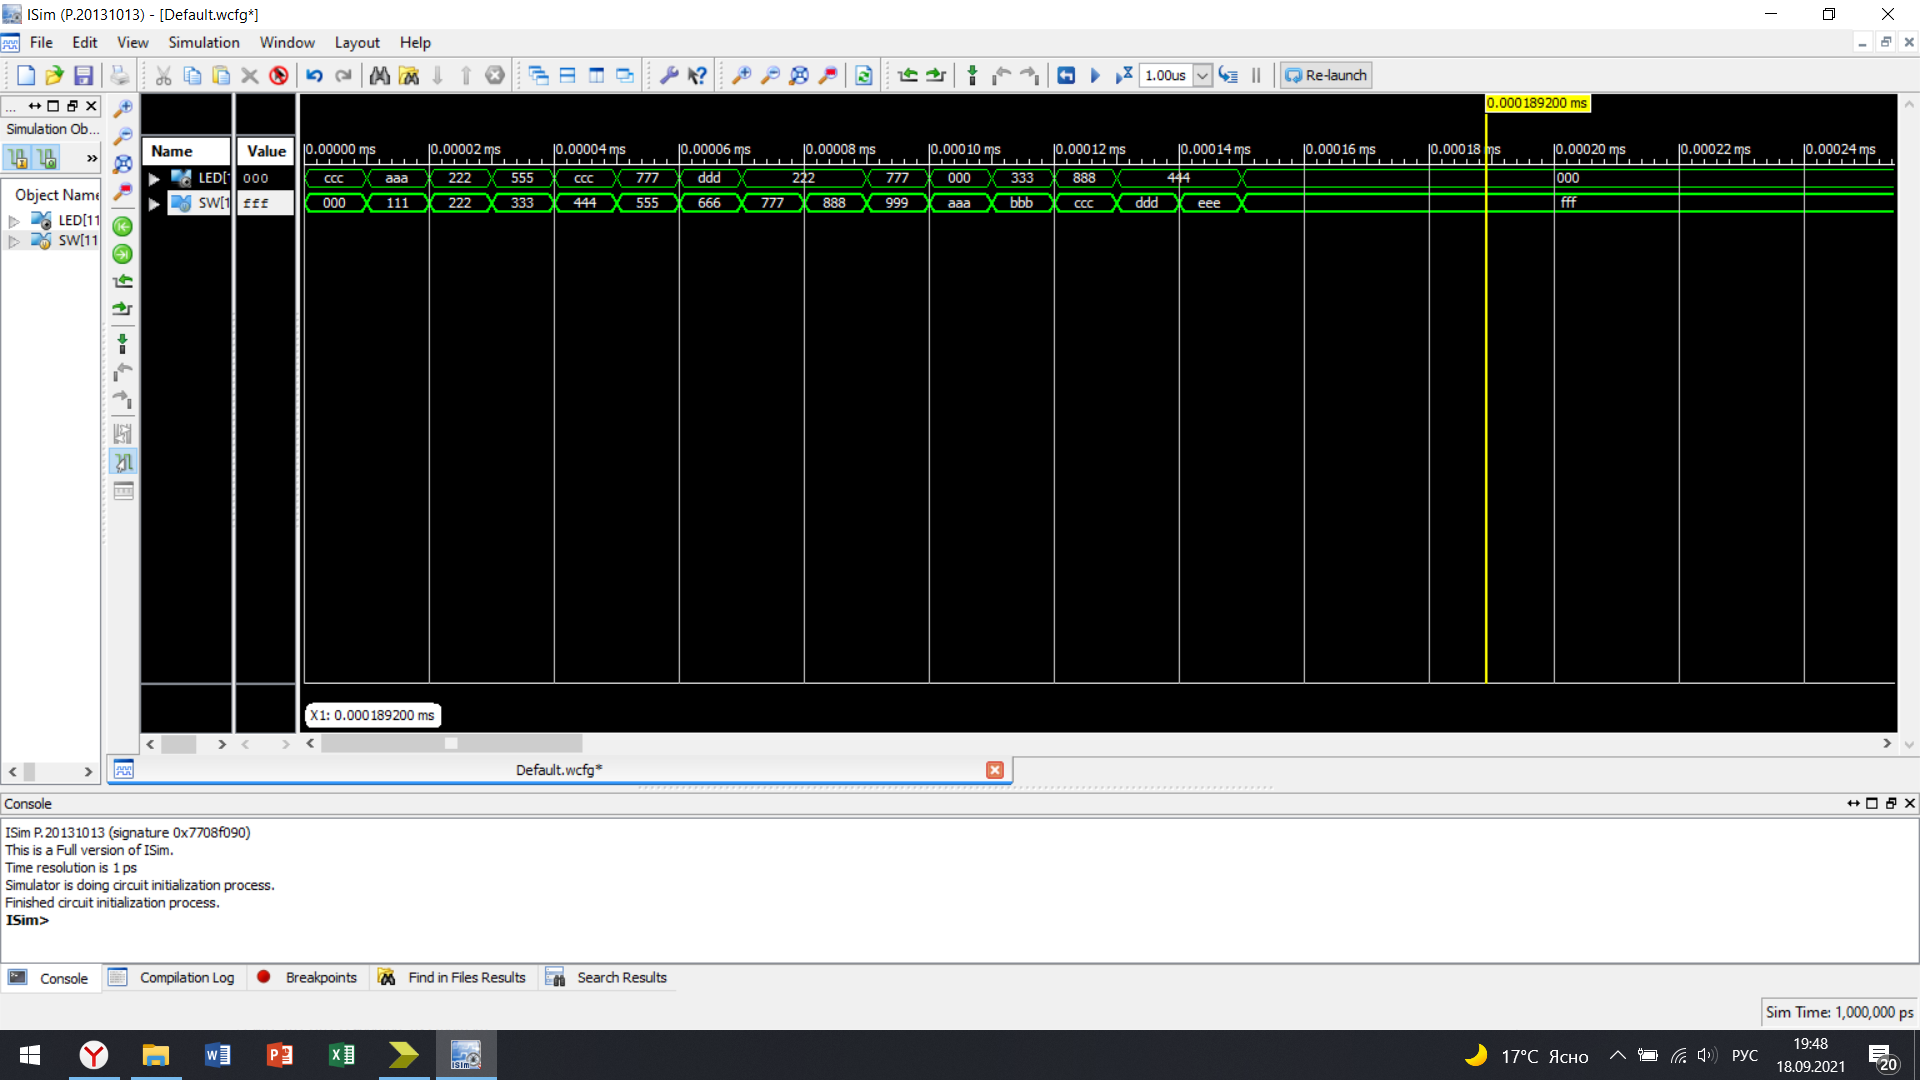
\includegraphics[width=\linewidth]{images/isim}
	\caption{Вывод iSim }
	\label{fig:isim}
\end{figure}

\newpage
\section{Вывод}
В ходе данной практической работы нами были получены общие навыки работы с программным обеспечением Xilinx ISE Design Suite, изучены основы языка Verilog. С помощью полученных знаний была спроектированы синтезируемые модели комбинационной схемы 4х4, описанной тремя различными способами.

\end{document}
